% Options for packages loaded elsewhere
\PassOptionsToPackage{unicode}{hyperref}
\PassOptionsToPackage{hyphens}{url}
%
\documentclass[
  12pt,
]{article}
\title{Git and GitHub inside RStudio}
\author{}
\date{\vspace{-2.5em}Fall 2021}

\usepackage{amsmath,amssymb}
\usepackage{lmodern}
\usepackage{iftex}
\ifPDFTeX
  \usepackage[T1]{fontenc}
  \usepackage[utf8]{inputenc}
  \usepackage{textcomp} % provide euro and other symbols
\else % if luatex or xetex
  \usepackage{unicode-math}
  \defaultfontfeatures{Scale=MatchLowercase}
  \defaultfontfeatures[\rmfamily]{Ligatures=TeX,Scale=1}
\fi
% Use upquote if available, for straight quotes in verbatim environments
\IfFileExists{upquote.sty}{\usepackage{upquote}}{}
\IfFileExists{microtype.sty}{% use microtype if available
  \usepackage[]{microtype}
  \UseMicrotypeSet[protrusion]{basicmath} % disable protrusion for tt fonts
}{}
\makeatletter
\@ifundefined{KOMAClassName}{% if non-KOMA class
  \IfFileExists{parskip.sty}{%
    \usepackage{parskip}
  }{% else
    \setlength{\parindent}{0pt}
    \setlength{\parskip}{6pt plus 2pt minus 1pt}}
}{% if KOMA class
  \KOMAoptions{parskip=half}}
\makeatother
\usepackage{xcolor}
\IfFileExists{xurl.sty}{\usepackage{xurl}}{} % add URL line breaks if available
\IfFileExists{bookmark.sty}{\usepackage{bookmark}}{\usepackage{hyperref}}
\hypersetup{
  pdftitle={Git and GitHub inside RStudio},
  hidelinks,
  pdfcreator={LaTeX via pandoc}}
\urlstyle{same} % disable monospaced font for URLs
\usepackage[margin=1in]{geometry}
\usepackage{graphicx}
\makeatletter
\def\maxwidth{\ifdim\Gin@nat@width>\linewidth\linewidth\else\Gin@nat@width\fi}
\def\maxheight{\ifdim\Gin@nat@height>\textheight\textheight\else\Gin@nat@height\fi}
\makeatother
% Scale images if necessary, so that they will not overflow the page
% margins by default, and it is still possible to overwrite the defaults
% using explicit options in \includegraphics[width, height, ...]{}
\setkeys{Gin}{width=\maxwidth,height=\maxheight,keepaspectratio}
% Set default figure placement to htbp
\makeatletter
\def\fps@figure{htbp}
\makeatother
\setlength{\emergencystretch}{3em} % prevent overfull lines
\providecommand{\tightlist}{%
  \setlength{\itemsep}{0pt}\setlength{\parskip}{0pt}}
\setcounter{secnumdepth}{-\maxdimen} % remove section numbering
\linespread{1.05} \usepackage{xcolor}
\ifLuaTeX
  \usepackage{selnolig}  % disable illegal ligatures
\fi

\begin{document}
\maketitle

We will be using \texttt{git} and \texttt{GitHub} to get send your
individual-based and team-based studies and get them back. In this short
tutorial, we will show you the process using \texttt{git} and
\texttt{GitHub} through \texttt{RStudio}. For that reason you have to
install \texttt{git} (the one most suitable for your operating system),
introduce your \texttt{GitHub} account to your local \texttt{git}, and
make sure \texttt{RStudio} can talk to local \texttt{git} (and,
therefore, \texttt{GitHub}). If you need assistance, I strongly suggest
you to take a look at the following great sources:

\begin{verbatim}
                        https://happygitwithr.com/ and
                        
                        https://ourcodingclub.github.io/tutorials/git/.
\end{verbatim}

We will create all individual-based and team-based assignments in
\texttt{GitHub} classroom of \texttt{MAT381E-Fall21} organization.


\includegraphics[width=1\linewidth]{images/organization} Afterwards, we
will send out you the assignment invitation links to you via Ninova
announcements so that you can join the assignment (you have to accept
the invitation to see the assignment repo under \texttt{MAT381E-Fall21}
organization). Once you accept the invitation, you will see that
\textbf{you have a repository under \texttt{MAT381E-Fall21} organization
for the relevant assignment}. For example
\texttt{\textless{}HW1-yourusername} for Homework 1. Please see my fake
student repo for HW 1.

\begin{figure}
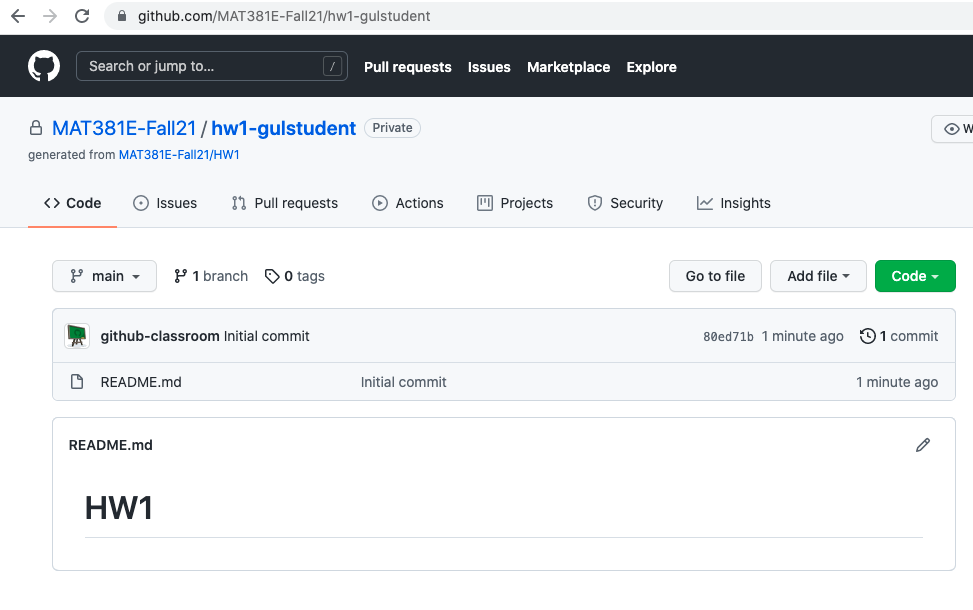
\includegraphics[width=1\linewidth]{images/github_gulstudent2} \end{figure}

Throughout the semester you will be an \textbf{outside collaborator} of
\texttt{MAT381E-Fall21} organization on GitHub, not a member. This means
that you can only see your repository under \texttt{MAT381E-Fall21}
organization, whereas I can see all the repositories.

In the ``repository URL'', copy the SSH URL of the assignment as shown
below (in my fake account, i did not take SSH key, but you should do,
otherwise you cannot commit and push your work from R Studio to GitHub)
:

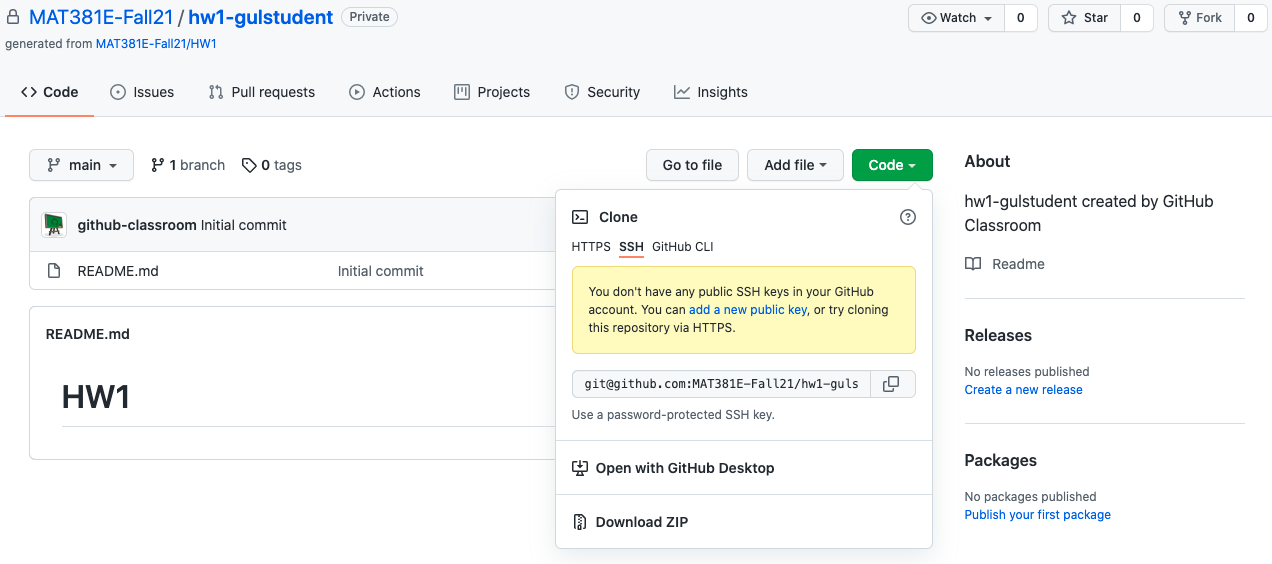
\includegraphics[width=1\linewidth]{images/green}

Then, in RStudio, start a new project:

\texttt{File\ \textgreater{}\ New\ Project\ \textgreater{}\ Version\ Control\ \textgreater{}\ Git}

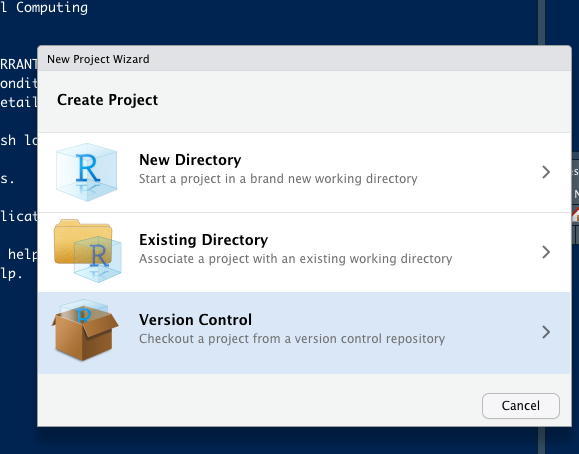
\includegraphics[width=1\linewidth]{images/git1}

Paste the URL of the assignment as shown below:

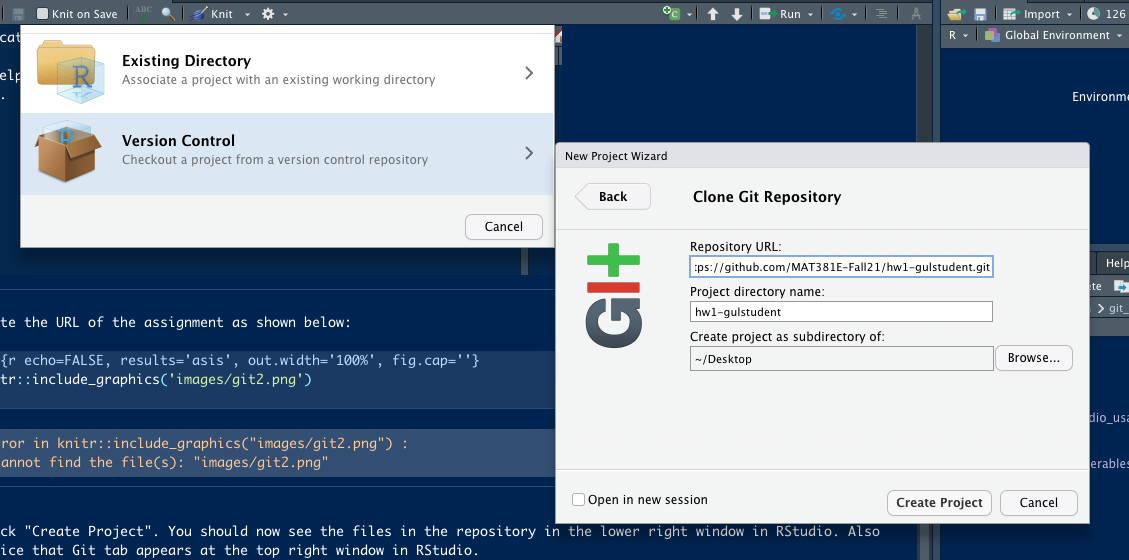
\includegraphics[width=1\linewidth]{images/git2}

Click ``Create Project''. You should now see the files in the repository
in the lower right window in RStudio. Also notice that Git tab appears
at the top right window in RStudio.

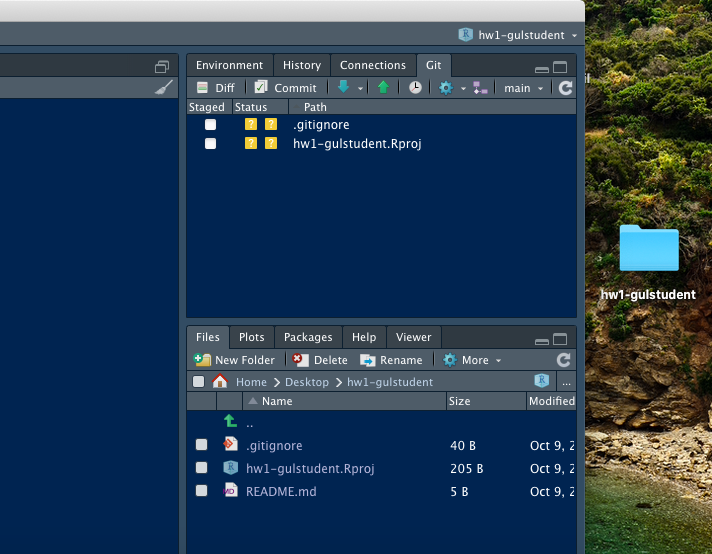
\includegraphics[width=1\linewidth]{images/git3}

Now, you have a local copy of your assignment. Work on it. Do whatever
you need. You can use Git tab to \texttt{commit} and \texttt{push}.

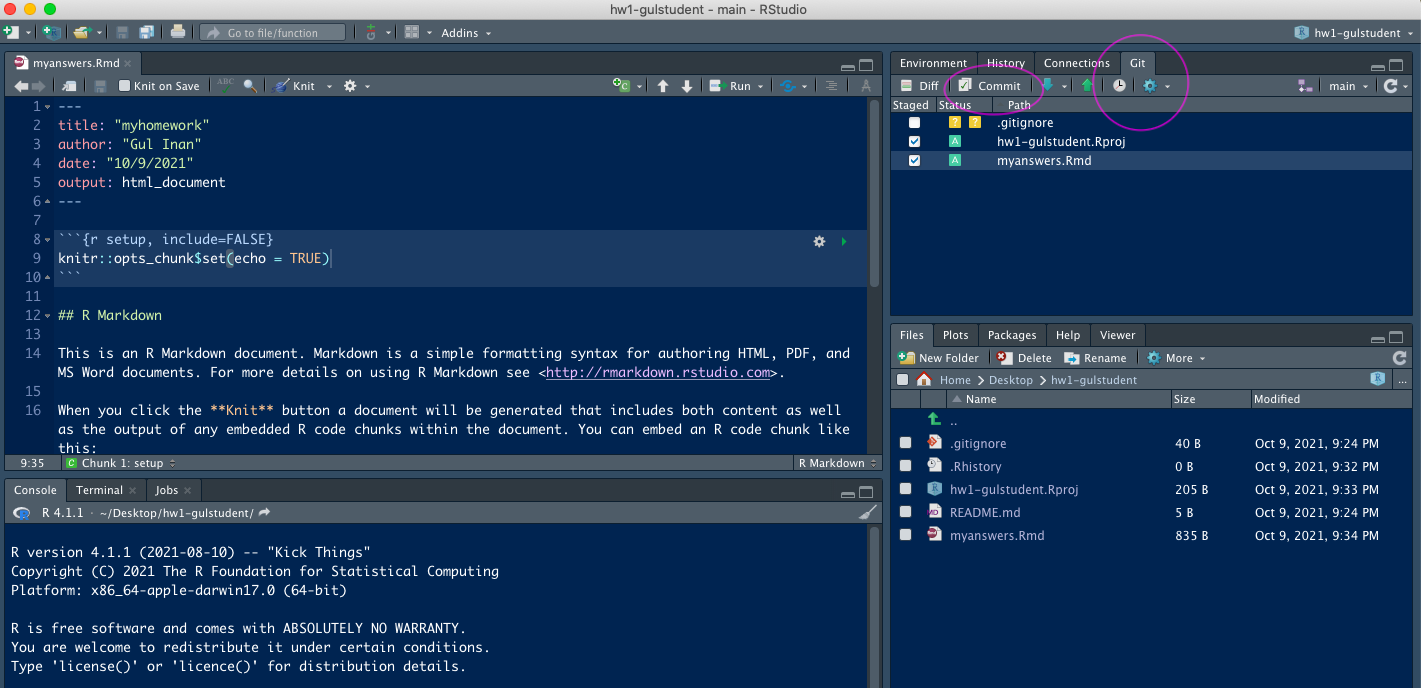
\includegraphics[width=1\linewidth]{images/commit1}
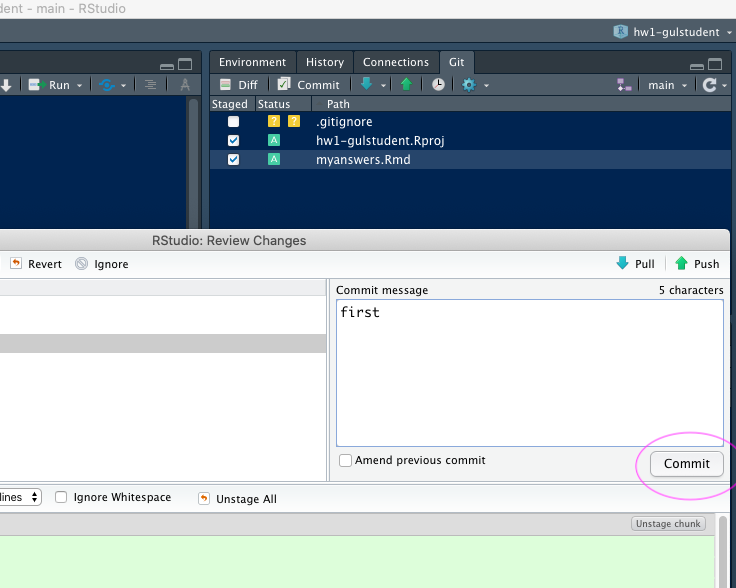
\includegraphics[width=1\linewidth]{images/commit2}
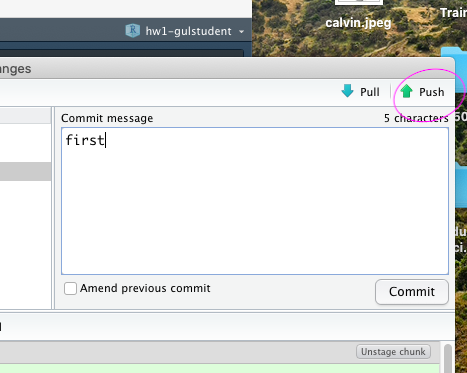
\includegraphics[width=1\linewidth]{images/push}

Check back your repository on GitHub!..Always send your assignments on
time!..(In the terminal window, use git commands \texttt{commit} and
\texttt{push} to send the changes you have done to your local repository
to GitHub.)

Wish you a productive semester!..

\begin{figure}

\includegraphics[width=1\linewidth]{images/github3} \end{figure}

\end{document}
